\section{Universal cover}

The following two theorems summarize our results about covering spaces.

\begin{theorem}[Galois Correspondence of Covering Spaces]
  There is a 1-1 correspondence between the subgroups of $\Gal(Y|X)$ and covers of $X$ that lie between $Y$ and $X$, given by the following maps
  \begin{align*}
    \{\mbox{ subgroups of $\Gal(Y|X)$ } \} &\longleftrightarrow  \{\mbox{ covers lying between $Y$ and $X$ } \}\\
    H &\longmapsto Y/H \\
    \Gal(Y|Z) & \longmapsfrom Z
  \end{align*}
  Under this correspondence, the normal subgroups of $\Gal(X|Y)$ correspond to Galois covers of $X$.
\end{theorem}

\begin{theorem}[Monodromy action of the fundamental group]
  \label{theorem:fundamentalGroupQuotient2}
  If $p:Y \rightarrow X$ is a Galois cover with $p(y) = x$, then there is a short exact sequence of groups
  \begin{equation*}
    \begin{tikzcd}
      1 \ar[r] & \pi_1(Y,y) \ar[r, "p_*"] & \pi_1(X,x) \ar[r,"M"] &  \Gal(Y|X) \ar[r] & 1
    \end{tikzcd}
  \end{equation*}
  where the map $p_*$ is sending a loop $\gamma$ in $Y$ to $p(\gamma)$ and $M$ is the monodromy action.
\end{theorem}

We will assume the following for now without proof.
\begin{theorem}[Existence of universal cover]
  For any space $X$, there exists a space $\widetilde{X}$ with a covering map $P:\widetilde{X} \rightarrow X$ satisfying the following properties:
  \begin{enumerate}
    \item $P$ is Galois.
    \item $\pi_1(\widetilde{X})$ is trivial. (We say that $\widetilde{X}$ is simply connected.)
    \item Every cover $Y$ of $X$ lies between $\widetilde{X}$ and $X$.
  \end{enumerate}
  Such a space $\widetilde{X}$ is called the \emph{universal cover} of $X$.
\end{theorem}

Several corrolaries follow immediately from this statement.












\subsection{Classification of all covers}



\begin{proposition}
  $\Gal(\widetilde{X} | X) \cong \pi_1(X,x)$.
\end{proposition}
\begin{proof}
  Apply Theorem \ref{theorem:fundamentalGroupQuotient2} to the cover $P:\widetilde{X} \rightarrow X$.
\end{proof}

\begin{theorem}[Galois correspondence \#2]
  \label{theorem:GaloisCorrespondence2}
  There is a 1-1 correspondence between the subgroups of $\pi_1(X,x)$ and covers of $X$, given by the following maps
  \begin{align*}
    \{\mbox{ subgroups of $\pi_1(X,x)$ } \} &\longleftrightarrow  \{\mbox{ covers of $X$ } \}\\
    H &\longmapsto \widetilde{X}/H \\
    \pi_1(Z,z) & \longmapsfrom Z
  \end{align*}
  Under this correspondence, the normal subgroups of $\pi_1(X,x)$ correspond to Galois covers of $X$.
\end{theorem}






\subsection{Subgroups of a free group}
Denote by $F_n$ the free group with $n$ generators.
\begin{theorem}
  Every subgroup of a finitely generated free group is free.
\end{theorem}
\begin{proof}
  Let $G = \mathrm{Free}(S)$ be a finitely generated free group with $|S|=k$.
  Let $X$ be a wedge of $k$ circles, so that $\pi_1(X) = G$.
  \begin{figure}[H]
    \centering
    \begin{tikzpicture}[scale=0.5]
     \begin{polaraxis}[grid=none, axis lines=none]
  \addplot[mark=none,domain=0:360,samples=300] {cos(x*5)};
\end{polaraxis}

    \end{tikzpicture}
    \caption{Wedge of 5 circles $\bigvee \limits_5 S^1$ has fundamental group $F_5$.}
  \end{figure}
  Every cover of $X$ is a graph, and the fundamental group of a graph is a free group (as there are no faces).
  Hence, by Theorem \ref{theorem:GaloisCorrespondence2} every subgroup of $G$ is free.
\end{proof}







\begin{theorem}
  If $F_m \triangleleft F_n$ then $n - 1 | m - 1$ and the index of $F_m$ inside $F_n$ is $(m-1)/(n-1)$.
\end{theorem}
\begin{proof}
  A normal subgroup $H$ of $G$ corresponds to a Galois cover $X$ of $\bigvee \limits_n S^1$, of some degree, say $d$.
  As $X$ is a cover, one can check by simple edge conting, that $X$ is free group on $(n-1)d + 1$ generators.
  The result follows.
\end{proof}









\subsection{Universal property of the universal cover}

We say that a space $Y$ is simply connected if $\pi_1(Y) \cong \set{\mathbb{1}}$.
\begin{proposition}
  Let $p:Y \rightarrow X$ be a Galois cover such that $Y$ is simply-connected.
  Further suppose that $p_2:Z \rightarrow X$ is another cover then $Z$ is a subcover of $Y$.
  \begin{equation*}
    \begin{tikzcd}
      Y \ar[rd, dashed, "\exists"] \ar[dd, "p"']\\
        & Z \ar[ld,"p_2"] \\
      X
    \end{tikzcd}
  \end{equation*}
\end{proposition}
\begin{proof}
  We will explicitly construct a map $p_1: Y \rightarrow Z$.
  Pick vertices $y_0$ in $Y$, $x_0$ in $X$, and $z_0$ in $Z$ such that $p(y_0) = x_0 = p_2(z_0)$.
  We define $p_1(y_0) = z_0$.

  Let $y$ be a vertex in $Y$. Let $\gamma$ be a path in $Y$.
  We push down $\gamma$ to X then lift it up to $X$ and set $p_1(y) = d_1 \widetilde{p(\gamma)}$.
  \begin{equation*}
    \begin{tikzcd}
      \gamma \ar[dd, mapsto]\\
        & \widetilde{p(\gamma)}  \\
      p(\gamma) \ar[ur, mapsto]
    \end{tikzcd}
  \end{equation*}

  We need to check that the map defined this way is well-defined i.e. it does not depend on the choice of the path $\gamma$.
  Suppose there are two paths $\gamma_1$ and $\gamma_2$ connecting $y_0$ to $y$.
  Then $\gamma_1^{-1} \gamma_2$ is a loop at $y$ and hence is (upto conjugation) a boundary of a face.
  It follows from this that the lifts of both $\gamma_1$ and $\gamma_2$ have the same endpoints.
\end{proof}


And so a universal cover of $X$ is any cover $\widetilde{X}$ of $X$ that is simply-connected.
There is a theorem of existence of the universal space of a general space, but in practice we simply construct these spaces by hand.

\begin{ex}
  The universal cover of $S^1$ is $\bbr^1$.
\end{ex}

\begin{ex}
  The universal cover of a cylinder (and hence also a Mobius strip) is $\bbr^1 \times [0,1]$.
\end{ex}

\begin{ex}
  The universal cover of a torus (and hence also a Klein bottle) is $\bbr^2$.
\end{ex}

\begin{ex}
  The universal cover of a real projective space is $S^2$.
\end{ex}

\begin{ex}
  The universal cover of a bouquet of $k$ circles is the Cayley graph of the free group with $k$ generators.
  \begin{figure}[H]
  \centering
    % \includegraphics[width=0.5\textwidth]{example-image}
    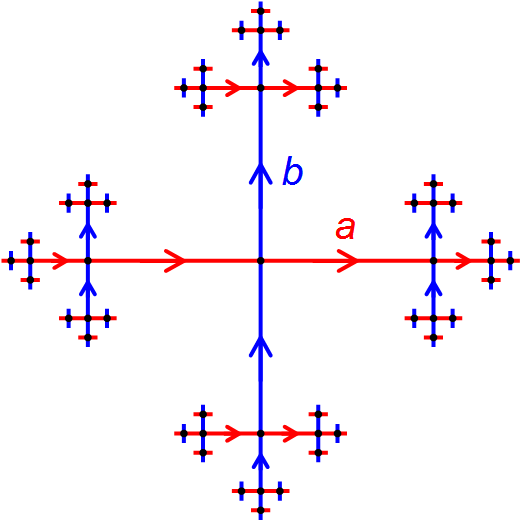
\includegraphics[width=0.5\textwidth]{CayleyF2.png}
    \caption{Universal cover of $F_2$}
  \end{figure}
\end{ex}

\begin{ex}
  A universal cover of a graph $X$ (space with no faces) can be constructed as follows:
  \begin{enumerate}
    \item Pick a vertex $x$.
    \item $\widetilde{X}$ is a graph whose vertices are paths in $X$ that start at $x$.
    \item There is an edge from $\gamma$ and $\gamma'$ if $\gamma = \gamma' \cdot e$ for some edge $e$.
    \item The covering map $P:\widetilde{X} \rightarrow X$ is the map $\gamma \mapsto d_1 \gamma$.
  \end{enumerate}
  \begin{qbox}
    Show that the $\widetilde{X}$ defined above is a simply-connected space and that $P$ is a covering map, and hence $\widetilde{X}$ is a universal cover.
  \end{qbox}
  This method can be generalized to spaces with faces. In this case, instead of taking all paths we need to take equivalence classes of paths with respect to boundaries of faces.
  \begin{equation*}
    \widetilde{X}_x = \set{ \mbox{paths starting at } x} / \mbox{faces}
  \end{equation*}
\end{ex}

\begin{remark}
  Finally, here is a comparison of the Galois correspondences for algebra and topology from Terrence Tao's blog \cite{TerrenceTao}.
  \begin{figure}[H]
  \centering
    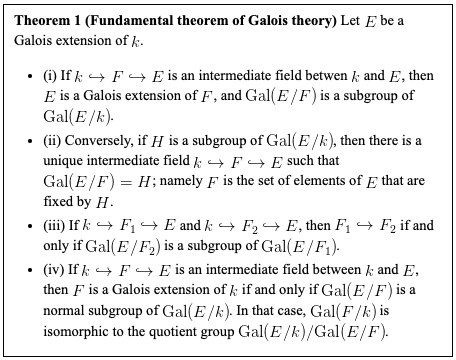
\includegraphics[width=0.8\textwidth]{TerryTao1.png}
    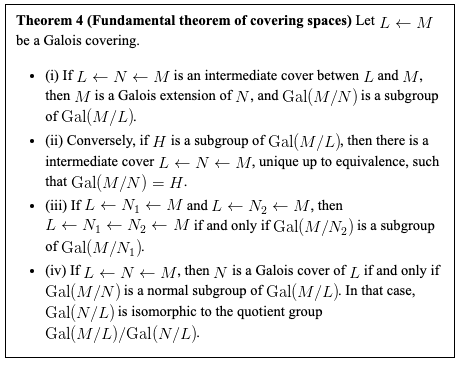
\includegraphics[width=0.8\textwidth]{TerryTao2.png}
  \end{figure}

\end{remark}

\begin{thebibliography}{9}
\bibitem{Szamuely}
Tam\'as Szamuely, \emph{Galois Groups and Fundamental Groups}, Cambridge Studies in Advanced Mathematics, 2007.

\bibitem{TerrenceTao}
Terrence Tao, \emph{Trying to understand the Galois correspondence},\\ \url{https://terrytao.wordpress.com/2018/08/28/trying-to-understand-the-galois-correspondence/}.
\end{thebibliography}


% In this section, we'll prove that for every (connected) space $Y$ and a vertex $y \in Y$, there exists a simply-connected space $\widetilde{Y}_y$ with a covering map
% \begin{align*}
%   \widetilde{Y}_y \rightarrow Y
% \end{align*}
%
% By Theorem \ref{theorem:liftingOfCovers} this cover is universal, in the sense that every cover $Z \rightarrow Y$ lies between $\widetilde{Y}_y$ and $Y$.
% \begin{equation*}
%   \begin{tikzcd}
%     & Z \ar[d] \\
%     \widetilde{Y}_y \ar[ur,"\exists !",dashrightarrow] \ar[r, "p'"']& Y
%   \end{tikzcd}
% \end{equation*}
%
% The following lemmas are more or less true by definition.
% \begin{lemma}
%   The fundamental group of a graph (=space with only vertices and edges) is a free group.
% \end{lemma}
%
% \begin{lemma}
%   Every cover of a graph is a graph.
% \end{lemma}
